\chapter{Metodologia}

A metodologia do presente trabalho é dividida em três principais partes. A primeira é a etapa de projeto dos componentes mecânicos que farão parte do satélite. Entre eles, as rodas de reação, motor DC (Direct Current - corrente contínua), mancal a ar e hastes. Também possui especificação dos componentes eletrônicos que constituirão o satélite. É na segunda etapa que ocorre a modelagem completa do sistema e especificações das limitações de movimentação do satélite, juntamente com a elaboração dos diagramas de blocos do controle. Nessa etapa também é feita a modelagem do motor DC, para que possamos fornecer torque para a planta sair da inércia. Já na terceira etapa, são abordados os elementos de software, de rede e supervisão do satélite. Nessa etapa também se encontram as especificações de software, desenvolvimento do software de controle e supervisão, juntamente com testes para validar as primeiras etapas.

%%%%%%%%%%%%%%%%%%%%%%%%%%%%%%%%%%%%%%%%%%%%%%%%%%%%%%%%%%%%%%%%%%%%%%
\section{Hardware}

Após a modelagem descrita no referencial teórico, pode-se modelar um simulador de satélite de fabricação factível.  O mancal a ar, a base de suporte do simulador do satélite, rodas de reação, motores Brushless (motor de corrente contínua sem escovas) e o outros elementos, podem ser vistos na imagem \ref{fig:satelite_completo}.

\begin{figure}[H]
  \caption{Desenho Mecânico do Satélite Completo}
  \begin{center}
      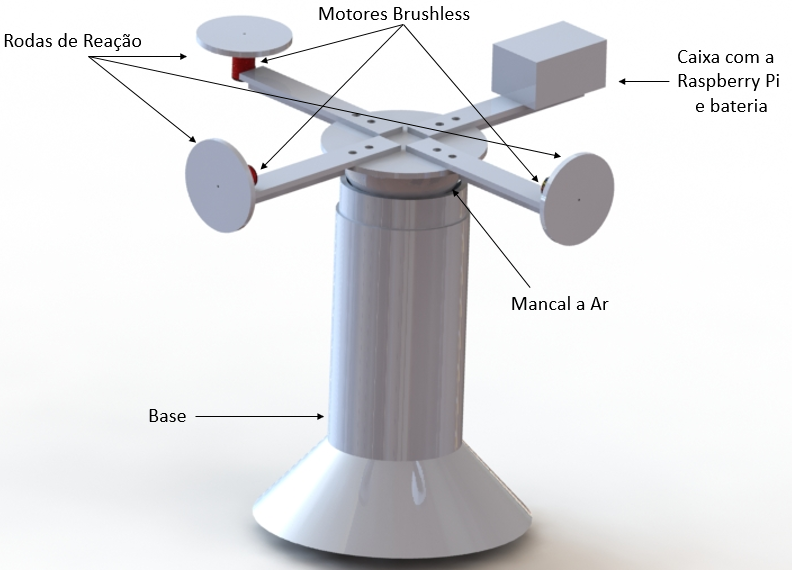
\includegraphics[scale=.6]{img/satelite_completo}
  \end{center}
  \fonte{Elaborado pelo Autor.} 
  \label{fig:satelite_completo}
\end{figure}

 Como podemos ver na imagem anterior, o modelo sofre várias simplificações em relação a um satélite real, onde o modelo passa a ser de fácil implementação, possibilitando a validação dos conceitos propostos nesse trabalho. Dentre várias simplificações, a mais óbvia, o simulador não apresentará de forma direta os movimentos de translação descritos no seção \ref{cap:dinamica}. Ainda, existe uma limitação para os ângulos $\phi$, $\theta$ e $\psi$ que é um intercalo de $0<\phi, \theta, \psi<240º$ devido a existência do mancal a ar e a simetria do corpo do satélite, como princípio para simplificar a modelagem matemática do mesmo.

Os principais elementos descritos na imagem anterior, serão descritos de forma detalhada na sequência, dentre eles o mancal a ar que pode ser visto na sequência.


%%%%%%%%%%%%%%%%%%%%%%%%%%%%%%%%%%%

\subsection{Mancal a Ar}

Um dos elementos mais importantes do simulador, é o mancal a ar. Ele possibilita a criação mínima de atrito entre a esfera e a região côncava, pois existe um fluxo de ar promovido por um sistema pneumático que cria uma camada de ar entre as duas partes. Com isso, a esfera fica com movimento praticamente livre de atritos dentro de uma região limitada pela geometria da esfera, o corpo do satélite, o peso do satélite e a pressão do sistema pneumático. O modelo mecânico do mancal com seus elementos podem ser visto na figura \ref{fig:base_desenho}.

\begin{figure}[H]
  \caption{Desenho Mecânico do Mancal a Ar}
  \begin{center}
      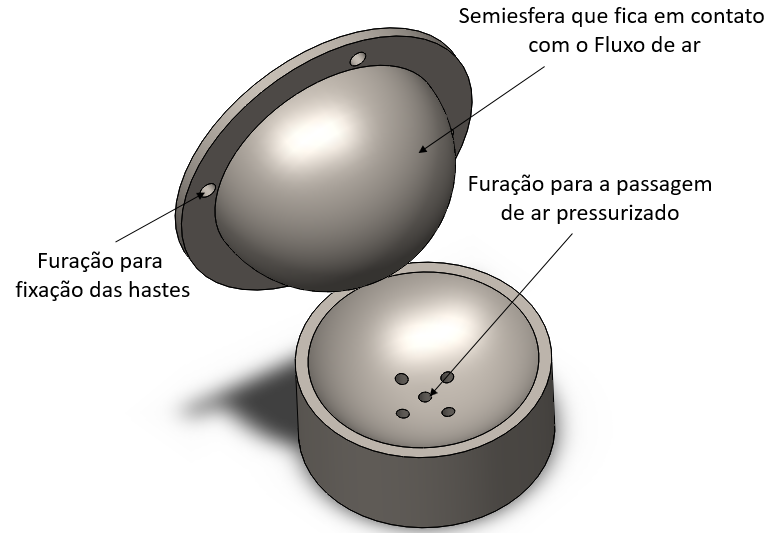
\includegraphics[scale=.45]{img/base_desenho}
  \end{center}
  \fonte{Elaborado pelo Autor.} 
  \label{fig:base_desenho}
\end{figure}

O mancal tem que ser usinado, deviso a precisão do encaixe entre a esfera e a região concava, para que a camada de ar seja o mais homogênea possível, evitando turbulências e regiões com atrito maior que outra. 

%%%%%%%%%%%%%%%%%%%%%%%%%%%%%%%%%%%
\subsection{Motor DC e Rodas de Reação}

O atuador do simulador de satélite será um conjunto de três motores Brushless dispostos sobre os três eixos cartesianos, com um motor em cada eixo. Juntamente com esses motores, são acopladas rodas de reação, que juntamente com s motores, farão os movimentos de rotação do satélite. Como vimos na imagem \ref{fig:satelite_completo}, os motores e as hastes estão distribuídos de forma simétrica e afastados do centro de massa do satélite, para facilitar a movimentação promovida pelo torque dos motores. Na imagem \ref{fig:motor_roda_desenho} podemos ver parte da haste, o motor e a roda de reação acoplados.

\begin{figure}[H]
  \caption{Desenho mecânico do conjunto Motor-Roda}
  \begin{center}
      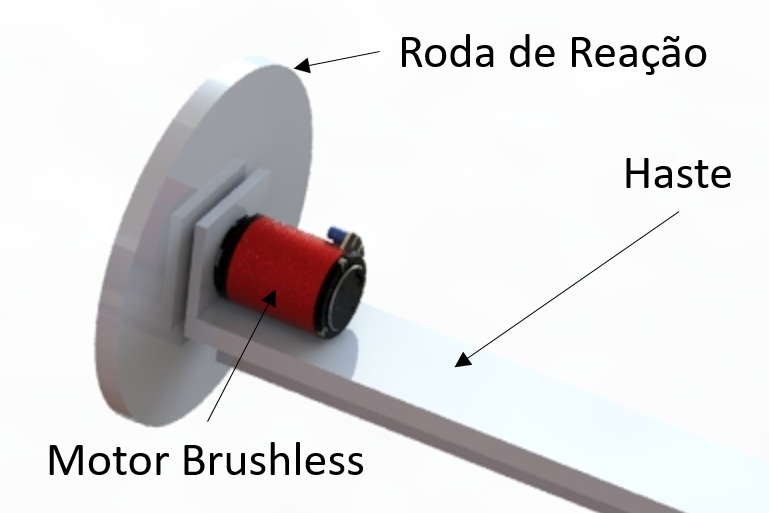
\includegraphics[scale=.45]{img/motor_roda_desenho}
  \end{center}
  \fonte{Elaborado pelo Autor.} 
  \label{fig:motor_roda_desenho}
\end{figure}

A roda de reação também deve ser usinada, pois precisamos de uma roda com uma massa e formato específico, para que possamos acoplar ao motor e o conjunto consiga realizar os movimentos propostos. 

%%%%%%%%%%%%%%%%%%%%%%%%%%%%%%%%%%%

\subsection{Elementos Eletrônicos}

A placa de desenvolvimento e prototipação de sistemas embarcados Raspberry Pi Zero W (Rpi) foi a escolhida, pois ela conta com os elementos mínimos de interfaceamento com os atuadores e outros periféricos. Além disso, ela possui conectividade através de um rede Wi-Fi, possibilitando a supervisão e controle do satélite, sem fio. Como o trabalho terá o seu desenvolvimento baseado em desenvolvimento de software e adaptações do sistema operacional, uma placa com suporte, boa documentação e comunidade ativa, facilita o desenvolvimento do trabalho. Uma representação dessa placa pode ser vista na figura \ref{fig:rasp_zero}

\begin{figure}[H]
  \caption{Raspberry Pi Zero}
  \begin{center}
      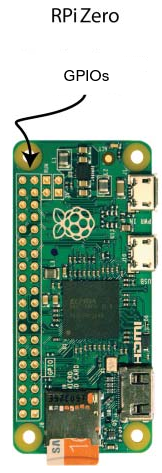
\includegraphics[scale=.55]{img/rasp_zero}
  \end{center}
  \fonte{Adaptado de \citeonline{Molloy2016}} 
  \label{fig:rasp_zero}
\end{figure}

Um outro elemento que será indispensável é o acelerômetro, o qual será o sensor de realimentação da posições angulares do satélite, sua comunicação com a RPi será através da interface I2C, que será descrita na seção de software. O acelerômetro informará o modelo da posição angular em graus, através da decomposição vetorial das acelerações nos eixos cartesianos, o uso de um acelerômetro posicionado no meio da planta evita o uso de um encoder (sensor de velocidade de rotação) em cada motor, além de ser mais acessível.

\begin{figure}[H]
  \caption{Circuito impresso com o acelerômetro MMA7260QT}
  \begin{center}
      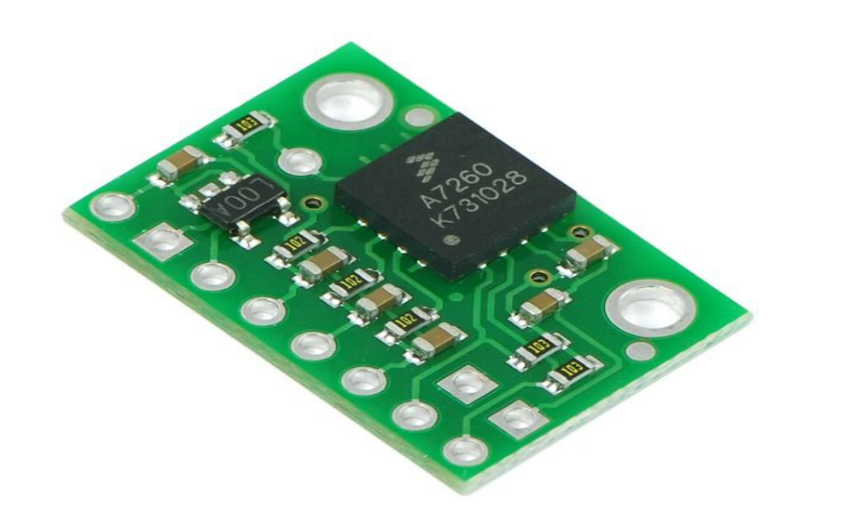
\includegraphics[scale=.4]{img/pci_acelerometro_calache_p22}
  \end{center}
  \fonte{Calache, Danilo Carreiro} 
  \label{fig:pci_acelerometro_calache_p22}
\end{figure}

Ainda, para o acionamento dos motores Brushless serão utilizados ESC (Electronic-Speed-Control - Controlador eletrônico de velocidade) que serão conectados com a bateria, os motores e a RPi. Com isso, todos os principais elementos de hardware foram descritos, sendo a modelagem dos mesmos o próximo passo do desenvolvimento.

%%%%%%%%%%%%%%%%%%%%%%%%%%%%%%%%%%%%%%%%%%%%%%%%%%%%%%%%%%%%%%%%%%%%%%

\section{Sistemas de Controle}

Após a descrição dos conceitos básicos de controle e do modelo mecânico do satélite, é possível desenvolver os modelos da planta e do sistema de controle. Na sequência será descrito a modelagem do motor de corrente contínua sugerido na seção anterior e posteriormente a modelagem completa do simulador de satélites.

%%%%%%%%%%%%%%%%%%%%%%%%%%%%%%%%%%%
\subsection{Modelo Motor DC}

Após a escolha do tipo de motor que será utilizado como atuador no controle da atitude do satélite, se faz necessário a modelagem do mesmo, para que consigamos acoplar ao modelo do satélite o torque que promoverá a variação mo momento angular do satélite, e por consequência, a posição angular. A figura \ref{fig:modelo_motor_dc} representa o modelo elétrico associado ao momento de inércia do rotor $J_{\omega 1}$ ao rotor e a da roda de reação $J_{\omega 2}$

\begin{figure}[H]
  \caption{Modelo do Motor DC}
  \begin{center}
      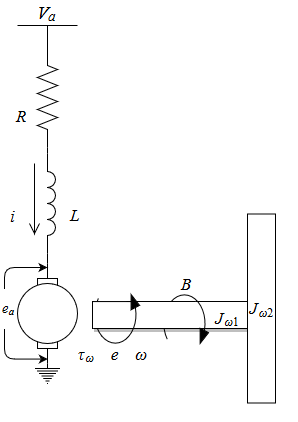
\includegraphics[scale=.7]{img/modelo_motor_dc}
  \end{center}
  \fonte{Elaborado pelo Autor.} 
  \label{fig:modelo_motor_dc}
\end{figure}

Onde $R_a$, $L_a$, $i_a$ e $e_a$ são a resistência, a indutância, a corrente e a tenção de armadura, respectivamente, $e_b$ é a tensão induzida e $\tau_{\omega}$ é o torque do motor. A relação que relaciona a corrente com a tensão de armadura pode ser vista na sequência \cite{Ogata}.

\begin{equation}
L_a \frac{di_a}{dt}+R_a i_a + e_b = e_a
\end{equation}

Como sabemos a relação entre a constante de torque $K_2$ e a tensão induzida, juntamente com a relação entre o ganho proporcional $K_1$ e a tensão da fonte $V_a$. Isso pode ser visto na sequência.

\begin{equation}
  e_a = K_2\frac{d\theta}{dt}
\end{equation}

e

\begin{equation}
  e_b = K_1V_a
\end{equation}

Temos que:

\begin{equation}\label{eq:la}
L_a \frac{di_a}{dt}+R_a i_a + K_2\frac{d\theta}{dt} = K_1V_a
\end{equation}

Ainda, a relação, que através do conceito de equilíbrio de torque, conseguimos relacionar o torque do motor $\tau_{\omega}$ com os momentos de inércia do rotor e da roda de reação com a corrente da armadura da seguinte forma:

\begin{equation}\label{eq:tauj}
\tau_{\omega} = (J_{\omega 1} + J_{\omega 2})\frac{d^{2}\theta}{dt^{2}}+B\frac{d\theta}{dt} = K_2 i_a
\end{equation}

Como queremos relacionar a tensão da fonte com o torque, devemos manipular as equações \ref{eq:la} e \ref{eq:tauj} e aplicarmos a transformada de Laplace. O resultado dessas operações pode ser visto na sequência: 

\begin{equation}
  \frac{\tau(s)}{V_a(s)} = \frac{K_1K_2}{(R_a+ sLa)(sJ+B)+K_1K_2}  
\end{equation}

Com isso modelamos o atuador do satélite, o próximo passo para a completa modelagem, é acoplar esse modelo com o do satélite descrito na seção \ref{cap:dinamica}. Esses paços serão descritos na próxima subseção.

\subsection{Modelo Completo do Satélite}

Como em partes, todo o satélite já foi modelado até agora, nessa subseção acoplaremos todos os modelo em um único, que terá como variável de interesse a posição angular tridimensional definida pelos ângulos de Euler $\psi, \theta, \phi$. Para a modelagem completa, usamos as equações que descevem o comportamento das rodas de ração, do motor Brushless e da própria dinâmica do satélite. Essa associação em forma de diagrama de blocos, malha aberta, pode ser visto na figura \ref{fig:modelo_satelite_malha_aberta}.

\begin{figure}[H]
  \caption{Modelo em malha aberta}
  \begin{center}
      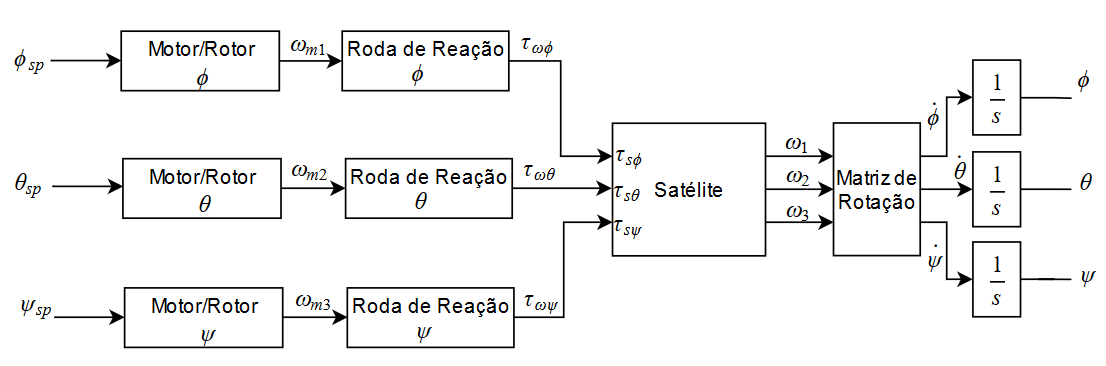
\includegraphics[scale=.55]{img/modelo_satelite_malha_aberta}
  \end{center}
  \fonte{Elaborado pelo Autor.} 
  \label{fig:modelo_satelite_malha_aberta}
\end{figure}

Se fecharmos a malha em posição, usando um acelerômetro e usarmos um controlador PID para o controle do torque do motor, por consequência, toda a dinâmica do satélite. O diagrama de blocos com realimentação e com o controlador PID pode ser visto na figura \ref{fig:modelo_satelite_pid}. 

\begin{figure}[H]
  \caption{Modelo em malha fechada com um Controlador PID}
  \begin{center}
      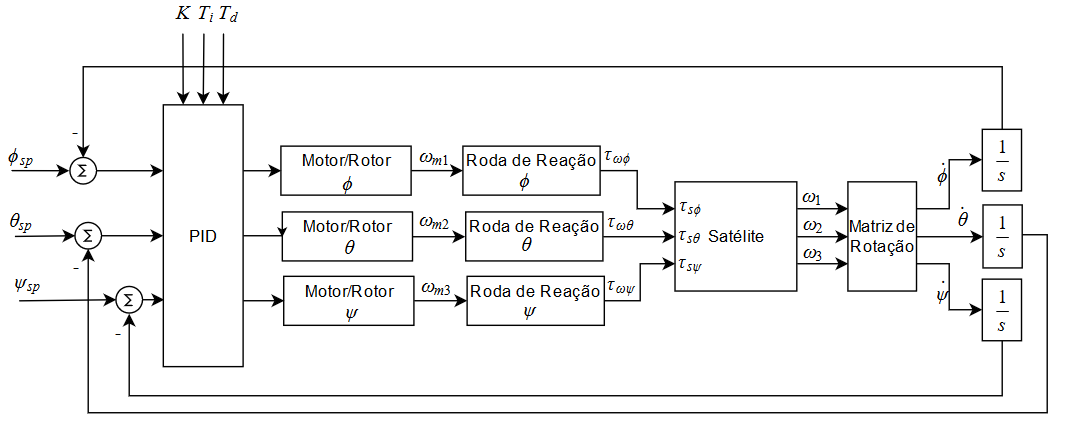
\includegraphics[scale=.58]{img/modelo_satelite_pid}
  \end{center}
  \fonte{Elaborado pelo Autor.} 
  \label{fig:modelo_satelite_pid}
\end{figure}

Esse último diagrama é usado para o desenvolvimento do controle em software, onde os parâmetros do controlador são estimados pelos diferentes tipos de sintonia descritos na revisão bibliográfica. Na sequência, serão descritos os métodos que serão utilizados para implementar esse modelo em Python e embarcar isso na RPi.


%%%%%%%%%%%%%%%%%%%%%%%%%%%%%%%%%%%%%%%%%%%%%%%%%%%%%%%%%%%%%%%%%%%%%%
\section{Software}

Após a modelagem, devemos implementar o modelo e configurar todas as interfaces com os atuadores e sistema supervisório. A figura \ref{fig:comunicacao_projeto} descreve muito bem a forma que se dará a comunicação entre os periféricos, através da interface I2C para a RPi se comunicar com ose ESC e o Protocolo MQTT para a comunicação com a supervisão.


\begin{figure}[H]
  \caption{Topologia de Rede}
  \begin{center}
      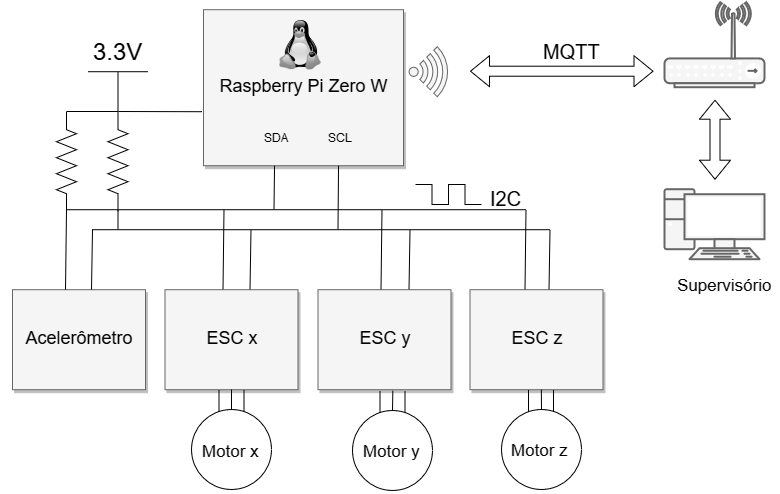
\includegraphics[scale=.75]{img/comunicacao_projeto}
  \end{center}
  \fonte{Elaborado pelo Autor.} 
  \label{fig:comunicacao_projeto}
\end{figure}

%%%%%%%%%%%%%%%%%%%%%%%%%%%%%%%%%%%
\subsection{Implementação do Controlador PID e Métodos de Sintonia}

Nessa etapa, ocorre a implementação usando a linguagem de programação Python, a qual, possui diversas bibliotecas de controle, interfaceamento e protocolos de comunicação. 

%%%%%%%%%%%%%%%%%%%%%%%%%%%%%%%%%%%
\subsection{Protocolos de Comunicação e Supervisório}

A comunicação entre os ESC e o acelerômetro será com I2C, pois facilita o uso de vários escravos com uma taxa de amostragem a priori, satisfatória. Já a comunicação com o supervisório, será usando um  o protocolo MQTT, o qual se popularizou na comunicação da internet das coisas (IoT - Internet of Things).

Com todos os itens especificados, podemos criar uma estimativa de tempo para a execução de cada parte principal do projeto. Isso pode ser visto no capítulo Cronograma.
